\documentclass[ignorenonframetext,]{beamer}
\setbeamertemplate{caption}[numbered]
\setbeamertemplate{caption label separator}{: }
\setbeamercolor{caption name}{fg=normal text.fg}
\beamertemplatenavigationsymbolsempty
\usepackage{lmodern}
\usepackage{amssymb,amsmath}
\usepackage{ifxetex,ifluatex}
\usepackage{fixltx2e} % provides \textsubscript
\ifnum 0\ifxetex 1\fi\ifluatex 1\fi=0 % if pdftex
  \usepackage[T1]{fontenc}
  \usepackage[utf8]{inputenc}
\else % if luatex or xelatex
  \ifxetex
    \usepackage{mathspec}
  \else
    \usepackage{fontspec}
  \fi
  \defaultfontfeatures{Ligatures=TeX,Scale=MatchLowercase}
    \setmainfont[]{IPAPMincho}
\fi
\usefonttheme{serif} % use mainfont rather than sansfont for slide text
% use upquote if available, for straight quotes in verbatim environments
\IfFileExists{upquote.sty}{\usepackage{upquote}}{}
% use microtype if available
\IfFileExists{microtype.sty}{%
\usepackage{microtype}
\UseMicrotypeSet[protrusion]{basicmath} % disable protrusion for tt fonts
}{}
\newif\ifbibliography
\hypersetup{
            pdftitle={Iteration - r4ds},
            pdfauthor={Tomoya Fukumoto},
            pdfborder={0 0 0},
            breaklinks=true}
\urlstyle{same}  % don't use monospace font for urls
\usepackage{color}
\usepackage{fancyvrb}
\newcommand{\VerbBar}{|}
\newcommand{\VERB}{\Verb[commandchars=\\\{\}]}
\DefineVerbatimEnvironment{Highlighting}{Verbatim}{commandchars=\\\{\}}
% Add ',fontsize=\small' for more characters per line
\usepackage{framed}
\definecolor{shadecolor}{RGB}{248,248,248}
\newenvironment{Shaded}{\begin{snugshade}}{\end{snugshade}}
\newcommand{\KeywordTok}[1]{\textcolor[rgb]{0.13,0.29,0.53}{\textbf{#1}}}
\newcommand{\DataTypeTok}[1]{\textcolor[rgb]{0.13,0.29,0.53}{#1}}
\newcommand{\DecValTok}[1]{\textcolor[rgb]{0.00,0.00,0.81}{#1}}
\newcommand{\BaseNTok}[1]{\textcolor[rgb]{0.00,0.00,0.81}{#1}}
\newcommand{\FloatTok}[1]{\textcolor[rgb]{0.00,0.00,0.81}{#1}}
\newcommand{\ConstantTok}[1]{\textcolor[rgb]{0.00,0.00,0.00}{#1}}
\newcommand{\CharTok}[1]{\textcolor[rgb]{0.31,0.60,0.02}{#1}}
\newcommand{\SpecialCharTok}[1]{\textcolor[rgb]{0.00,0.00,0.00}{#1}}
\newcommand{\StringTok}[1]{\textcolor[rgb]{0.31,0.60,0.02}{#1}}
\newcommand{\VerbatimStringTok}[1]{\textcolor[rgb]{0.31,0.60,0.02}{#1}}
\newcommand{\SpecialStringTok}[1]{\textcolor[rgb]{0.31,0.60,0.02}{#1}}
\newcommand{\ImportTok}[1]{#1}
\newcommand{\CommentTok}[1]{\textcolor[rgb]{0.56,0.35,0.01}{\textit{#1}}}
\newcommand{\DocumentationTok}[1]{\textcolor[rgb]{0.56,0.35,0.01}{\textbf{\textit{#1}}}}
\newcommand{\AnnotationTok}[1]{\textcolor[rgb]{0.56,0.35,0.01}{\textbf{\textit{#1}}}}
\newcommand{\CommentVarTok}[1]{\textcolor[rgb]{0.56,0.35,0.01}{\textbf{\textit{#1}}}}
\newcommand{\OtherTok}[1]{\textcolor[rgb]{0.56,0.35,0.01}{#1}}
\newcommand{\FunctionTok}[1]{\textcolor[rgb]{0.00,0.00,0.00}{#1}}
\newcommand{\VariableTok}[1]{\textcolor[rgb]{0.00,0.00,0.00}{#1}}
\newcommand{\ControlFlowTok}[1]{\textcolor[rgb]{0.13,0.29,0.53}{\textbf{#1}}}
\newcommand{\OperatorTok}[1]{\textcolor[rgb]{0.81,0.36,0.00}{\textbf{#1}}}
\newcommand{\BuiltInTok}[1]{#1}
\newcommand{\ExtensionTok}[1]{#1}
\newcommand{\PreprocessorTok}[1]{\textcolor[rgb]{0.56,0.35,0.01}{\textit{#1}}}
\newcommand{\AttributeTok}[1]{\textcolor[rgb]{0.77,0.63,0.00}{#1}}
\newcommand{\RegionMarkerTok}[1]{#1}
\newcommand{\InformationTok}[1]{\textcolor[rgb]{0.56,0.35,0.01}{\textbf{\textit{#1}}}}
\newcommand{\WarningTok}[1]{\textcolor[rgb]{0.56,0.35,0.01}{\textbf{\textit{#1}}}}
\newcommand{\AlertTok}[1]{\textcolor[rgb]{0.94,0.16,0.16}{#1}}
\newcommand{\ErrorTok}[1]{\textcolor[rgb]{0.64,0.00,0.00}{\textbf{#1}}}
\newcommand{\NormalTok}[1]{#1}
\usepackage{longtable,booktabs}
\usepackage{caption}
% These lines are needed to make table captions work with longtable:
\makeatletter
\def\fnum@table{\tablename~\thetable}
\makeatother
\usepackage{graphicx,grffile}
\makeatletter
\def\maxwidth{\ifdim\Gin@nat@width>\linewidth\linewidth\else\Gin@nat@width\fi}
\def\maxheight{\ifdim\Gin@nat@height>\textheight0.8\textheight\else\Gin@nat@height\fi}
\makeatother
% Scale images if necessary, so that they will not overflow the page
% margins by default, and it is still possible to overwrite the defaults
% using explicit options in \includegraphics[width, height, ...]{}
\setkeys{Gin}{width=\maxwidth,height=\maxheight,keepaspectratio}

% Prevent slide breaks in the middle of a paragraph:
\widowpenalties 1 10000
\raggedbottom

\AtBeginPart{
  \let\insertpartnumber\relax
  \let\partname\relax
  \frame{\partpage}
}
\AtBeginSection{
  \ifbibliography
  \else
    \let\insertsectionnumber\relax
    \let\sectionname\relax
    \frame{\sectionpage}
  \fi
}
\AtBeginSubsection{
  \let\insertsubsectionnumber\relax
  \let\subsectionname\relax
  \frame{\subsectionpage}
}

\setlength{\parindent}{0pt}
\setlength{\parskip}{6pt plus 2pt minus 1pt}
\setlength{\emergencystretch}{3em}  % prevent overfull lines
\providecommand{\tightlist}{%
  \setlength{\itemsep}{0pt}\setlength{\parskip}{0pt}}
\setcounter{secnumdepth}{0}
\usepackage{zxjatype}
\usepackage[ipa]{zxjafont}

\title{Iteration - r4ds}
\author{Tomoya Fukumoto}
\date{2019-09-06}

\begin{document}
\frame{\titlepage}

\begin{frame}{Iteration}

繰り返し作業をどうやって自動化するための二つの手法

\begin{enumerate}
\def\labelenumi{\arabic{enumi}.}
\tightlist
\item
  ループ
\item
  関数型プログラミング(functional programming)
\end{enumerate}

\end{frame}

\begin{frame}[fragile]{準備}

\begin{Shaded}
\begin{Highlighting}[]
\KeywordTok{library}\NormalTok{(tidyverse)}
\end{Highlighting}
\end{Shaded}

ループに関わるのは\texttt{base}ライブラリ

FPに関わるのは\texttt{purrr}ライブラリ

\end{frame}

\begin{frame}{21.2 For loops}

最も標準的なループ

\end{frame}

\begin{frame}[fragile]{例:各行のmedianを求める(ループなし)}

\begin{Shaded}
\begin{Highlighting}[]
\NormalTok{df <-}\StringTok{ }\KeywordTok{tibble}\NormalTok{(}
         \DataTypeTok{a =} \KeywordTok{rnorm}\NormalTok{(}\DecValTok{10}\NormalTok{),}
         \DataTypeTok{b =} \KeywordTok{rnorm}\NormalTok{(}\DecValTok{10}\NormalTok{),}
         \DataTypeTok{c =} \KeywordTok{rnorm}\NormalTok{(}\DecValTok{10}\NormalTok{),}
         \DataTypeTok{d =} \KeywordTok{rnorm}\NormalTok{(}\DecValTok{10}\NormalTok{)}
\NormalTok{) }
\KeywordTok{median}\NormalTok{(df}\OperatorTok{$}\NormalTok{a)}
\KeywordTok{median}\NormalTok{(df}\OperatorTok{$}\NormalTok{b)}
\KeywordTok{median}\NormalTok{(df}\OperatorTok{$}\NormalTok{c)}
\KeywordTok{median}\NormalTok{(df}\OperatorTok{$}\NormalTok{d)}
\end{Highlighting}
\end{Shaded}

\end{frame}

\begin{frame}[fragile]{例:各行のmedianを求める(ループ)}

\begin{Shaded}
\begin{Highlighting}[]
\NormalTok{output <-}\StringTok{ }\KeywordTok{vector}\NormalTok{(}\StringTok{"double"}\NormalTok{, }\KeywordTok{ncol}\NormalTok{(df))  }\CommentTok{# 1. output}
\ControlFlowTok{for}\NormalTok{ (i }\ControlFlowTok{in} \KeywordTok{seq_along}\NormalTok{(df)) \{            }\CommentTok{# 2. sequence}
\NormalTok{  output[[i]] <-}\StringTok{ }\KeywordTok{median}\NormalTok{(df[[i]])      }\CommentTok{# 3. body}
\NormalTok{\}}
\NormalTok{output}
\end{Highlighting}
\end{Shaded}

\begin{verbatim}
## [1] -0.2082671 -0.3499398 -0.4117896 -0.3206133
\end{verbatim}

\end{frame}

\begin{frame}[fragile]{ループの構成要素 output}

\begin{Shaded}
\begin{Highlighting}[]
\NormalTok{output <-}\StringTok{ }\KeywordTok{vector}\NormalTok{(}\StringTok{"double"}\NormalTok{, }\KeywordTok{ncol}\NormalTok{(df))}
\end{Highlighting}
\end{Shaded}

\begin{itemize}
\tightlist
\item
  ループの出力の器
\item
  ループが始まる前に作る
\item
  \texttt{vector}関数で型と長さを指定する
\item
  長さを指定しないと処理が遅くなる
\end{itemize}

\end{frame}

\begin{frame}[fragile]{ループの構成要素 sequence}

\begin{Shaded}
\begin{Highlighting}[]
\NormalTok{i }\ControlFlowTok{in} \KeywordTok{seq_along}\NormalTok{(df)}
\end{Highlighting}
\end{Shaded}

\begin{itemize}
\tightlist
\item
  どうループを回すか
\item
  一周するたびに\texttt{i}がベクトル\texttt{seq\_along(df)}の中で値を変化させる
\item
  \texttt{seq\_along(df)}は\texttt{1:length(df)}と\textbf{ほぼ}同じ

  \begin{itemize}
  \tightlist
  \item
    今回は\texttt{c(1,2,3,4)}
  \item
    \texttt{length(df)}が\texttt{0}のときだけ違う
  \end{itemize}
\end{itemize}

\end{frame}

\begin{frame}[fragile]{ループの構成要素 body}

\begin{Shaded}
\begin{Highlighting}[]
\NormalTok{output[[i]] <-}\StringTok{ }\KeywordTok{median}\NormalTok{(df[[i]])}
\end{Highlighting}
\end{Shaded}

\begin{itemize}
\tightlist
\item
  ループで実際に処理する内容

  \begin{itemize}
  \tightlist
  \item
    1回目は\texttt{output{[}{[}1{]}{]}\ \textless{}-\ median(df{[}{[}1{]}{]})}
  \item
    2回目は\texttt{output{[}{[}2{]}{]}\ \textless{}-\ median(df{[}{[}2{]}{]})}
  \item
    \ldots{}
  \end{itemize}
\end{itemize}

\end{frame}

\begin{frame}{21.2.1 Exercises}

1を見てみる

\end{frame}

\begin{frame}{21.3 For loop variations}

\begin{enumerate}
\def\labelenumi{\arabic{enumi}.}
\tightlist
\item
  オブジェクトを修正するループ(作成するのではなく)
\item
  要素の名前や値で回すループ(インデックスではなく)
\item
  出力の長さが不明の場合
\item
  ループ回数が不明の場合
\end{enumerate}

\end{frame}

\begin{frame}[fragile]{21.3.1 Modifying an existing object}

\begin{Shaded}
\begin{Highlighting}[]
\NormalTok{df <-}\StringTok{ }\KeywordTok{tibble}\NormalTok{(}\DataTypeTok{a =} \KeywordTok{rnorm}\NormalTok{(}\DecValTok{10}\NormalTok{), }\DataTypeTok{b =} \KeywordTok{rnorm}\NormalTok{(}\DecValTok{10}\NormalTok{), }\DataTypeTok{c =} \KeywordTok{rnorm}\NormalTok{(}\DecValTok{10}\NormalTok{), }\DataTypeTok{d =} \KeywordTok{rnorm}\NormalTok{(}\DecValTok{10}\NormalTok{))}
\NormalTok{rescale01 <-}\StringTok{ }\ControlFlowTok{function}\NormalTok{(x) \{}
\NormalTok{    rng <-}\StringTok{ }\KeywordTok{range}\NormalTok{(x, }\DataTypeTok{na.rm =} \OtherTok{TRUE}\NormalTok{)}
\NormalTok{  (x }\OperatorTok{-}\StringTok{ }\NormalTok{rng[}\DecValTok{1}\NormalTok{]) }\OperatorTok{/}\StringTok{ }\NormalTok{(rng[}\DecValTok{2}\NormalTok{] }\OperatorTok{-}\StringTok{ }\NormalTok{rng[}\DecValTok{1}\NormalTok{])}
\NormalTok{\} }
\NormalTok{df}\OperatorTok{$}\NormalTok{a <-}\StringTok{ }\KeywordTok{rescale01}\NormalTok{(df}\OperatorTok{$}\NormalTok{a)}
\NormalTok{df}\OperatorTok{$}\NormalTok{b <-}\StringTok{ }\KeywordTok{rescale01}\NormalTok{(df}\OperatorTok{$}\NormalTok{b)}
\NormalTok{df}\OperatorTok{$}\NormalTok{c <-}\StringTok{ }\KeywordTok{rescale01}\NormalTok{(df}\OperatorTok{$}\NormalTok{c)}
\NormalTok{df}\OperatorTok{$}\NormalTok{d <-}\StringTok{ }\KeywordTok{rescale01}\NormalTok{(df}\OperatorTok{$}\NormalTok{d)}
\end{Highlighting}
\end{Shaded}

\begin{block}{等価}

\begin{Shaded}
\begin{Highlighting}[]
\ControlFlowTok{for}\NormalTok{ (i }\ControlFlowTok{in} \KeywordTok{seq_along}\NormalTok{(df)) \{}
\NormalTok{    df[[i]] <-}\StringTok{ }\KeywordTok{rescale01}\NormalTok{(df[[i]])}
\NormalTok{\}}
\end{Highlighting}
\end{Shaded}

\end{block}

\end{frame}

\begin{frame}[fragile]{21.3.2 Looping patterns}

ループを回すときのsequenceの作法

\begin{enumerate}
\def\labelenumi{\arabic{enumi}.}
\tightlist
\item
  \texttt{for\ (i\ in\ seq\_along(xs))}
  インデックスとして1から順に数え上げる

  \begin{itemize}
  \tightlist
  \item
    最も一般的かつ汎用的
  \end{itemize}
\item
  \texttt{for\ (x\ in\ xs)} ベクトル\texttt{xs}の要素を一つずつとる

  \begin{itemize}
  \tightlist
  \item
    出力を保存しにくい

    \begin{itemize}
    \tightlist
    \item
      オブジェクト操作でなく副作用(plot, writeなど)に使う
    \end{itemize}
  \end{itemize}
\item
  \texttt{for\ (nm\ in\ names(xs))} 要素の名前を一つずつとる

  \begin{itemize}
  \tightlist
  \item
    要素の名前を使いたい場合

    \begin{itemize}
    \tightlist
    \item
      plotのタイトルとか
    \end{itemize}
  \end{itemize}
\end{enumerate}

\end{frame}

\begin{frame}[fragile]{インデックスを使った方法が最も汎用的}

インデックスを使った方法は他の2つをシミュレートできる

\begin{Shaded}
\begin{Highlighting}[]
\ControlFlowTok{for}\NormalTok{ (i }\ControlFlowTok{in} \KeywordTok{seq_along}\NormalTok{(x)) \{}
\NormalTok{  name <-}\StringTok{ }\KeywordTok{names}\NormalTok{(x)[[i]]}
\NormalTok{  value <-}\StringTok{ }\NormalTok{x[[i]]}
\NormalTok{\}}
\end{Highlighting}
\end{Shaded}

\end{frame}

\begin{frame}{21.3.3 Unknown output length}

ループする前に出力の長さがわからないとき

\end{frame}

\begin{frame}[fragile]{乱数でベクトルの長さが変わる場合}

\begin{block}{ダメな例}

\begin{Shaded}
\begin{Highlighting}[]
\NormalTok{means <-}\StringTok{ }\KeywordTok{c}\NormalTok{(}\DecValTok{0}\NormalTok{, }\DecValTok{1}\NormalTok{, }\DecValTok{2}\NormalTok{)}
\NormalTok{output <-}\StringTok{ }\KeywordTok{double}\NormalTok{()}
\ControlFlowTok{for}\NormalTok{ (i }\ControlFlowTok{in} \KeywordTok{seq_along}\NormalTok{(means)) \{}
\NormalTok{  n <-}\StringTok{ }\KeywordTok{sample}\NormalTok{(}\DecValTok{100}\NormalTok{, }\DecValTok{1}\NormalTok{)}
\NormalTok{  output <-}\StringTok{ }\KeywordTok{c}\NormalTok{(output, }\KeywordTok{rnorm}\NormalTok{(n, means[[i]]))}
\NormalTok{\}}
\end{Highlighting}
\end{Shaded}

毎回全データコピーするので\(O(n^2)\)の計算量がかかる

\end{block}

\end{frame}

\begin{frame}[fragile]{良い例}

\begin{Shaded}
\begin{Highlighting}[]
\NormalTok{out <-}\StringTok{ }\KeywordTok{vector}\NormalTok{(}\StringTok{"list"}\NormalTok{, }\KeywordTok{length}\NormalTok{(means))}
\ControlFlowTok{for}\NormalTok{ (i }\ControlFlowTok{in} \KeywordTok{seq_along}\NormalTok{(means)) \{}
\NormalTok{  n <-}\StringTok{ }\KeywordTok{sample}\NormalTok{(}\DecValTok{100}\NormalTok{, }\DecValTok{1}\NormalTok{)}
\NormalTok{  out[[i]] <-}\StringTok{ }\KeywordTok{rnorm}\NormalTok{(n, means[[i]])}
\NormalTok{\}}
\NormalTok{output <-}\StringTok{ }\KeywordTok{unlist}\NormalTok{(out)}
\end{Highlighting}
\end{Shaded}

\begin{block}{他の例}

\begin{itemize}
\tightlist
\item
  \texttt{paste(out,\ x)}と追加していくのではなく、\texttt{out}をまとめて作ったあと\texttt{paste(out,\ collapse=TRUE)}でくっつける
\item
  データフレームの行を追加していくのではなく、リストで作って\texttt{bind\_rows(output)}でくっつける
\end{itemize}

\end{block}

\end{frame}

\begin{frame}{21.3.4 Unknown sequence length}

事前にループする回数がわからないとき

\end{frame}

\begin{frame}[fragile]{\texttt{while}}

\begin{Shaded}
\begin{Highlighting}[]
\ControlFlowTok{while}\NormalTok{ (condition)\{}
  \CommentTok{#body}
\NormalTok{\}}
\end{Highlighting}
\end{Shaded}

シミュレーションでよく使う

\begin{itemize}
\tightlist
\item
  精度が出るまで反復する、とか
\end{itemize}

\end{frame}

\begin{frame}{21.3.5 Exercises}

\end{frame}

\begin{frame}{21.4 For loops vs.~functionals}

関数型プログラミングとは

\end{frame}

\begin{frame}[fragile]{for loopを使った例}

\begin{Shaded}
\begin{Highlighting}[]
\NormalTok{df <-}\StringTok{ }\KeywordTok{tibble}\NormalTok{(}\DataTypeTok{a =} \KeywordTok{rnorm}\NormalTok{(}\DecValTok{10}\NormalTok{),}
         \DataTypeTok{b =} \KeywordTok{rnorm}\NormalTok{(}\DecValTok{10}\NormalTok{),}
         \DataTypeTok{c =} \KeywordTok{rnorm}\NormalTok{(}\DecValTok{10}\NormalTok{),}
         \DataTypeTok{d =} \KeywordTok{rnorm}\NormalTok{(}\DecValTok{10}\NormalTok{))}

\NormalTok{output <-}\StringTok{ }\KeywordTok{vector}\NormalTok{(}\StringTok{"double"}\NormalTok{, }\KeywordTok{length}\NormalTok{(df))}
\ControlFlowTok{for}\NormalTok{ (i }\ControlFlowTok{in} \KeywordTok{seq_along}\NormalTok{(df)) \{}
\NormalTok{    output[[i]] <-}\StringTok{ }\KeywordTok{mean}\NormalTok{(df[[i]])}
\NormalTok{\}}
\NormalTok{output}
\end{Highlighting}
\end{Shaded}

\begin{verbatim}
## [1]  0.04440174 -0.64643055 -0.06354274 -0.68199421
\end{verbatim}

\end{frame}

\begin{frame}[fragile]{何回も使いそうだから関数にする}

\begin{Shaded}
\begin{Highlighting}[]
\NormalTok{col_mean <-}\StringTok{ }\ControlFlowTok{function}\NormalTok{(df) \{}
\NormalTok{    output <-}\StringTok{ }\KeywordTok{vector}\NormalTok{(}\StringTok{"double"}\NormalTok{, }\KeywordTok{length}\NormalTok{(df))}
  \ControlFlowTok{for}\NormalTok{ (i }\ControlFlowTok{in} \KeywordTok{seq_along}\NormalTok{(df)) \{}
\NormalTok{        output[i] <-}\StringTok{ }\KeywordTok{mean}\NormalTok{(df[[i]])}
\NormalTok{    \}}
\NormalTok{    output}
\NormalTok{\}}
\end{Highlighting}
\end{Shaded}

\end{frame}

\begin{frame}[fragile]{平均以外の集計でも使うだろう}

\begin{Shaded}
\begin{Highlighting}[]
\NormalTok{col_median <-}\StringTok{ }\ControlFlowTok{function}\NormalTok{(df) \{}
\NormalTok{    output <-}\StringTok{ }\KeywordTok{vector}\NormalTok{(}\StringTok{"double"}\NormalTok{, }\KeywordTok{length}\NormalTok{(df))}
  \ControlFlowTok{for}\NormalTok{ (i }\ControlFlowTok{in} \KeywordTok{seq_along}\NormalTok{(df)) \{}
\NormalTok{        output[i] <-}\StringTok{ }\KeywordTok{median}\NormalTok{(df[[i]])}
\NormalTok{    \}}
\NormalTok{    output}
\NormalTok{\}}
\NormalTok{col_sd <-}\StringTok{ }\ControlFlowTok{function}\NormalTok{(df) \{}
\NormalTok{    output <-}\StringTok{ }\KeywordTok{vector}\NormalTok{(}\StringTok{"double"}\NormalTok{, }\KeywordTok{length}\NormalTok{(df))}
  \ControlFlowTok{for}\NormalTok{ (i }\ControlFlowTok{in} \KeywordTok{seq_along}\NormalTok{(df)) \{}
\NormalTok{        output[i] <-}\StringTok{ }\KeywordTok{sd}\NormalTok{(df[[i]])}
\NormalTok{    \}}
\NormalTok{    output}
\NormalTok{\}}
\end{Highlighting}
\end{Shaded}

二回以上のコピペをしてしまった!

\end{frame}

\begin{frame}[fragile]{関数型プログラミング}

\begin{Shaded}
\begin{Highlighting}[]
\NormalTok{col_summary <-}\StringTok{ }\ControlFlowTok{function}\NormalTok{(df, fun) \{}
\NormalTok{    out <-}\StringTok{ }\KeywordTok{vector}\NormalTok{(}\StringTok{"double"}\NormalTok{, }\KeywordTok{length}\NormalTok{(df))}
  \ControlFlowTok{for}\NormalTok{ (i }\ControlFlowTok{in} \KeywordTok{seq_along}\NormalTok{(df)) \{}
\NormalTok{        out[i] <-}\StringTok{ }\KeywordTok{fun}\NormalTok{(df[[i]])}
\NormalTok{    \}}
\NormalTok{    out}
\NormalTok{\}}
\KeywordTok{col_summary}\NormalTok{(df, median)}
\KeywordTok{col_summary}\NormalTok{(df, sd)}
\end{Highlighting}
\end{Shaded}

Rでは関数の引数として関数を渡すことができる

\(\Rightarrow\)関数型プログラミング

\end{frame}

\begin{frame}{21.4.1 Exercises}

1,2

\end{frame}

\begin{frame}[fragile]{21.5 The map functions}

for loopをfunctionalで置き換える関数\texttt{purrr::map}

\end{frame}

\begin{frame}[fragile]{\texttt{purrr::map}}

\begin{block}{Usage}

\begin{Shaded}
\begin{Highlighting}[]
\KeywordTok{map}\NormalTok{(.x, .f, ...)}
\end{Highlighting}
\end{Shaded}

\end{block}

\begin{block}{Arguments}

\begin{longtable}[]{@{}ll@{}}
\toprule
\textbf{.x} & listかatomic vector\tabularnewline
\textbf{.f} & 関数かformula\tabularnewline
\textbf{\ldots{}} &
関数に渡すパラメータ。たとえば\texttt{na.rm\ =\ TRUE}\tabularnewline
\bottomrule
\end{longtable}

\end{block}

\begin{block}{return}

ベクトル\texttt{.x}の要素をそれぞれ関数\texttt{.f}に適用し、その結果をリストで返す

\end{block}

\end{frame}

\begin{frame}[fragile]{Example 1}

\begin{Shaded}
\begin{Highlighting}[]
\NormalTok{sheets <-}\StringTok{ }\KeywordTok{c}\NormalTok{( }\StringTok{"(NAP)全国"}\NormalTok{,}
        \StringTok{"(NAP)関西"}\NormalTok{,}
        \StringTok{"(NAP)関西以外"}\NormalTok{)}

\NormalTok{poo <-}\StringTok{ }\KeywordTok{map}\NormalTok{(sheets,}
\NormalTok{       read_excel,}
       \DataTypeTok{path =} \StringTok{"input/★【weekly】POO_Flex_Histrical_Data.xlsx"}\NormalTok{,}
       \DataTypeTok{trim_ws =}\NormalTok{ F)}
\end{Highlighting}
\end{Shaded}

\end{frame}

\begin{frame}[fragile]{\texttt{map}一族}

戻り値をリストではない形式に変換して返すこともできる

\begin{itemize}
\tightlist
\item
  \texttt{map} makes a list.
\item
  \texttt{map\_lgl} makes a logical vector.
\item
  \texttt{map\_int} makes an integer vector.
\item
  \texttt{map\_dbl} makes a double vector.
\item
  \texttt{map\_chr} makes a character vector.
\item
  \texttt{map\_df} makes a dataframe \textbf{特に重要}
\end{itemize}

これらが使えるかは\texttt{.f}の戻り値しだい

\end{frame}

\begin{frame}[fragile]{Example 2}

\begin{Shaded}
\begin{Highlighting}[]
\NormalTok{    data_all <-}\StringTok{ }\KeywordTok{left_join}\NormalTok{(data_used_mean,data_used_sgm,}\DataTypeTok{by=}\NormalTok{grp) }\OperatorTok\StringTok{ }
\StringTok{      }\KeywordTok{left_join}\NormalTok{(data_used_sgm2,}\DataTypeTok{by=}\NormalTok{grp) }\OperatorTok\StringTok{       }
\StringTok{      }\KeywordTok{left_join}\NormalTok{(data_used_max,}\DataTypeTok{by=}\NormalTok{grp) }\OperatorTok\StringTok{ }
\StringTok{      }\KeywordTok{right_join}\NormalTok{(data_used_att,}\DataTypeTok{by=}\NormalTok{grp) }\OperatorTok\StringTok{ }
\StringTok{      }\KeywordTok{map_df}\NormalTok{(prod_chkin) }\CommentTok{#xベクトル内の全ての要素に対して関数prod_chkinを適用するイメージ}
\end{Highlighting}
\end{Shaded}

\texttt{prod\_chkin}はdataframeの各変数をベクトルからベクトルに変換する関数

\end{frame}

\begin{frame}{\texttt{map}でやると何がいいのか}

\begin{itemize}
\tightlist
\item
  読みやすい、書きやすい

  \begin{itemize}
  \tightlist
  \item
    ループは本来処理したいことに対して余計なモノが多すぎる
  \end{itemize}
\item
  処理が早い

  \begin{itemize}
  \tightlist
  \item
    と昔は言われていたが今はそうでもないらしい
  \item
    内部的にはCで処理しているから少し早い
  \end{itemize}
\end{itemize}

\end{frame}

\begin{frame}[fragile]{21.5.1 Shortcuts}

\texttt{map}を使う上でのテクニック

\end{frame}

\begin{frame}[fragile]{余裕のあるやり方}

関数を定義する

\begin{Shaded}
\begin{Highlighting}[]
\NormalTok{mylm <-}\StringTok{ }\ControlFlowTok{function}\NormalTok{(df)\{}
  \KeywordTok{lm}\NormalTok{(mpg }\OperatorTok{~}\StringTok{ }\NormalTok{wt, }\DataTypeTok{data =}\NormalTok{ df)}
\NormalTok{\}}
\NormalTok{models <-}\StringTok{ }\NormalTok{mtcars }\OperatorTok
\StringTok{  }\KeywordTok{split}\NormalTok{(.}\OperatorTok{$}\NormalTok{cyl) }\OperatorTok
\StringTok{  }\KeywordTok{map}\NormalTok{(mylm)}
\end{Highlighting}
\end{Shaded}

\end{frame}

\begin{frame}[fragile]{せっかちなやり方}

\begin{block}{無名関数}

\begin{Shaded}
\begin{Highlighting}[]
\NormalTok{models <-}\StringTok{ }\NormalTok{mtcars }\OperatorTok
\StringTok{  }\KeywordTok{split}\NormalTok{(.}\OperatorTok{$}\NormalTok{cyl) }\OperatorTok
\StringTok{  }\KeywordTok{map}\NormalTok{(}\ControlFlowTok{function}\NormalTok{(df)}\KeywordTok{lm}\NormalTok{(mpg }\OperatorTok{~}\StringTok{ }\NormalTok{wt, }\DataTypeTok{data =}\NormalTok{ df))}
\end{Highlighting}
\end{Shaded}

\end{block}

\begin{block}{formula}

\begin{Shaded}
\begin{Highlighting}[]
\NormalTok{models <-}\StringTok{ }\NormalTok{mtcars }\OperatorTok
\StringTok{  }\KeywordTok{split}\NormalTok{(.}\OperatorTok{$}\NormalTok{cyl) }\OperatorTok
\StringTok{  }\KeywordTok{map}\NormalTok{(}\OperatorTok{~}\KeywordTok{lm}\NormalTok{(mpg }\OperatorTok{~}\StringTok{ }\NormalTok{wt, }\DataTypeTok{data =}\NormalTok{ .))}
\end{Highlighting}
\end{Shaded}

\end{block}

\end{frame}

\begin{frame}[fragile]{リストの各要素から情報を取り出す}

\begin{Shaded}
\begin{Highlighting}[]
\NormalTok{models }\OperatorTok\StringTok{ }
\StringTok{  }\KeywordTok{map}\NormalTok{(summary) }\OperatorTok\StringTok{ }
\StringTok{  }\KeywordTok{map_dbl}\NormalTok{(}\OperatorTok{~}\NormalTok{.}\OperatorTok{$}\NormalTok{r.squared)}
\end{Highlighting}
\end{Shaded}

\begin{verbatim}
##         4         6         8 
## 0.5086326 0.4645102 0.4229655
\end{verbatim}

\begin{block}{shortcut}

\begin{Shaded}
\begin{Highlighting}[]
\NormalTok{models }\OperatorTok
\StringTok{  }\KeywordTok{map}\NormalTok{(summary) }\OperatorTok
\StringTok{  }\KeywordTok{map_dbl}\NormalTok{(}\StringTok{"r.squared"}\NormalTok{)}
\end{Highlighting}
\end{Shaded}

\end{block}

\end{frame}

\begin{frame}[fragile]{21.5.2 BaseR}

\texttt{lapply}, \texttt{sapply},
\texttt{vapply}という関数がbaseにある。

\texttt{map}を学べば不要

\end{frame}

\begin{frame}{21.5.3 Exercises}

全部自分でやらなければ身につかない

\end{frame}

\begin{frame}[fragile]{21.6 Dealing with failure}

\texttt{map}関数を使ったプログラムのデバッグ技術

\texttt{map}中に一つエラーがあると全部出力しなくてむかつく

\begin{block}{for programmer}

例外処理

\end{block}

\end{frame}

\begin{frame}[fragile]{\texttt{purrr::safely}}

関数\texttt{safely}は関数\texttt{.f}を引数として、\texttt{.f}を修正した関数を返す。

修正された関数は必ず長さ2のリストを返す関数で、その戻り値は下記の通り

\begin{enumerate}
\def\labelenumi{\arabic{enumi}.}
\tightlist
\item
  要素\texttt{result}は元々の関数\texttt{.f}の結果。ただしその結果がエラーだった場合は\texttt{NULL}
\item
  要素\texttt{error}はエラーオブジェクト。\texttt{.f}の結果がエラーでなければ\texttt{NULL}
\end{enumerate}

\end{frame}

\begin{frame}[fragile]{Example 1}

\begin{Shaded}
\begin{Highlighting}[]
\NormalTok{safe_log <-}\StringTok{ }\KeywordTok{safely}\NormalTok{(log)}
\KeywordTok{safe_log}\NormalTok{(}\DecValTok{10}\NormalTok{)}
\end{Highlighting}
\end{Shaded}

\begin{verbatim}
## $result
## [1] 2.302585
## 
## $error
## NULL
\end{verbatim}

\begin{Shaded}
\begin{Highlighting}[]
\KeywordTok{safe_log}\NormalTok{(}\StringTok{"a"}\NormalTok{)}
\end{Highlighting}
\end{Shaded}

\begin{verbatim}
## $result
## NULL
## 
## $error
## <simpleError in .Primitive("log")(x, base): non-numeric argument to mathematical function>
\end{verbatim}

\end{frame}

\begin{frame}[fragile]{Example 2}

\begin{Shaded}
\begin{Highlighting}[]
\NormalTok{x <-}\StringTok{ }\KeywordTok{list}\NormalTok{(}\DecValTok{1}\NormalTok{, }\DecValTok{10}\NormalTok{, }\StringTok{"a"}\NormalTok{)}
\NormalTok{y <-}\StringTok{ }\NormalTok{x }\OperatorTok\StringTok{ }\KeywordTok{map}\NormalTok{(}\KeywordTok{safely}\NormalTok{(log))}
\KeywordTok{str}\NormalTok{(y)}
\end{Highlighting}
\end{Shaded}

\begin{verbatim}
## List of 3
##  $ :List of 2
##   ..$ result: num 0
##   ..$ error : NULL
##  $ :List of 2
##   ..$ result: num 2.3
##   ..$ error : NULL
##  $ :List of 2
##   ..$ result: NULL
##   ..$ error :List of 2
##   .. ..$ message: chr "non-numeric argument to mathematical function"
##   .. ..$ call   : language .Primitive("log")(x, base)
##   .. ..- attr(*, "class")= chr [1:3] "simpleError" "error" "condition"
\end{verbatim}

\end{frame}

\begin{frame}[fragile]{\texttt{purrr::transpose}}

関数\texttt{transpose}でもっと見易く

\begin{Shaded}
\begin{Highlighting}[]
\NormalTok{y <-}\StringTok{ }\NormalTok{y }\OperatorTok\StringTok{ }\NormalTok{transpose}
\KeywordTok{str}\NormalTok{(y)}
\end{Highlighting}
\end{Shaded}

\begin{verbatim}
## List of 2
##  $ result:List of 3
##   ..$ : num 0
##   ..$ : num 2.3
##   ..$ : NULL
##  $ error :List of 3
##   ..$ : NULL
##   ..$ : NULL
##   ..$ :List of 2
##   .. ..$ message: chr "non-numeric argument to mathematical function"
##   .. ..$ call   : language .Primitive("log")(x, base)
##   .. ..- attr(*, "class")= chr [1:3] "simpleError" "error" "condition"
\end{verbatim}

\end{frame}

\begin{frame}[fragile]{一族 \texttt{purrr::possibly}}

関数\texttt{.f}がエラーのときに返す値を第二引数に指定できる。

\begin{Shaded}
\begin{Highlighting}[]
\NormalTok{possibly_log <-}\StringTok{ }\KeywordTok{possibly}\NormalTok{(log, }\OtherTok{NA}\NormalTok{)}
\KeywordTok{possibly_log}\NormalTok{(}\DecValTok{10}\NormalTok{)}
\end{Highlighting}
\end{Shaded}

\begin{verbatim}
## [1] 2.302585
\end{verbatim}

\begin{Shaded}
\begin{Highlighting}[]
\KeywordTok{possibly_log}\NormalTok{(}\StringTok{"a"}\NormalTok{)}
\end{Highlighting}
\end{Shaded}

\begin{verbatim}
## [1] NA
\end{verbatim}

全くエラーを返さなくなる

\end{frame}

\begin{frame}[fragile]{21.7 Mapping over multiple arguments}

複数入力の\texttt{map}

\end{frame}

\begin{frame}[fragile]{\texttt{purrr::map2}}

\begin{block}{Usage}

\begin{Shaded}
\begin{Highlighting}[]
\KeywordTok{map2}\NormalTok{(.x, .y, .f, ...)}
\end{Highlighting}
\end{Shaded}

\end{block}

\begin{block}{Arguments}

\begin{longtable}[]{@{}ll@{}}
\toprule
\textbf{.x} & listかatomic vector\tabularnewline
\textbf{.y} & listかatomic
vector。.xと.yとのそれぞれのベクトルの長さが同じでなければならない\tabularnewline
\textbf{.f} & 関数かformula\tabularnewline
\textbf{\ldots{}} &
関数に渡すパラメータ。たとえば\texttt{na.rm\ =\ TRUE}\tabularnewline
\bottomrule
\end{longtable}

\end{block}

\begin{block}{return}

ベクトル\texttt{.x},\texttt{.y}の要素をそれぞれ関数\texttt{.f}に適用し、その結果をリストで返す

\end{block}

\end{frame}

\begin{frame}[fragile]{Example}

\begin{Shaded}
\begin{Highlighting}[]
\NormalTok{mu <-}\StringTok{ }\KeywordTok{list}\NormalTok{(}\DecValTok{5}\NormalTok{, }\DecValTok{10}\NormalTok{, }\OperatorTok{-}\DecValTok{3}\NormalTok{)}
\NormalTok{sigma <-}\StringTok{ }\KeywordTok{list}\NormalTok{(}\DecValTok{1}\NormalTok{, }\DecValTok{5}\NormalTok{, }\DecValTok{10}\NormalTok{)}
\KeywordTok{map2}\NormalTok{(mu, sigma, rnorm, }\DataTypeTok{n =} \DecValTok{5}\NormalTok{)}
\end{Highlighting}
\end{Shaded}

\begin{verbatim}
## [[1]]
## [1] 5.489210 5.734225 3.690561 5.714282 4.897131
## 
## [[2]]
## [1] 13.599892  4.208838 12.638960  6.875779 26.941896
## 
## [[3]]
## [1]  -2.985130 -11.045972  -9.563942   1.819610 -10.467585
\end{verbatim}

\end{frame}

\begin{frame}{Visualization of map2}

\begin{figure}
\centering
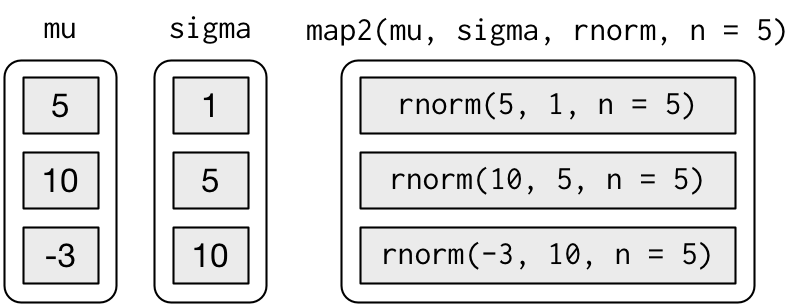
\includegraphics{../img/lists-map2.png}
\caption{structure of map2}
\end{figure}

\end{frame}

\begin{frame}[fragile]{\texttt{purrr::pmap}}

入力が3つ以上の場合

\begin{Shaded}
\begin{Highlighting}[]
\NormalTok{n <-}\StringTok{ }\KeywordTok{list}\NormalTok{(}\DecValTok{1}\NormalTok{, }\DecValTok{3}\NormalTok{, }\DecValTok{5}\NormalTok{)}
\NormalTok{args2 <-}\StringTok{ }\KeywordTok{list}\NormalTok{(}\DataTypeTok{mean =}\NormalTok{ mu, }\DataTypeTok{sd =}\NormalTok{ sigma, }\DataTypeTok{n =}\NormalTok{ n)}
\NormalTok{args2 }\OperatorTok\StringTok{ }\KeywordTok{pmap}\NormalTok{(rnorm) }\OperatorTok\StringTok{ }\KeywordTok{str}\NormalTok{()}
\end{Highlighting}
\end{Shaded}

\begin{verbatim}
## List of 3
##  $ : num 4.17
##  $ : num [1:3] 0.442 7.228 4.561
##  $ : num [1:5] 3.988 4.514 -0.806 1.765 -5.19
\end{verbatim}

\end{frame}

\begin{frame}{Visualization of pmap}

\begin{figure}
\centering
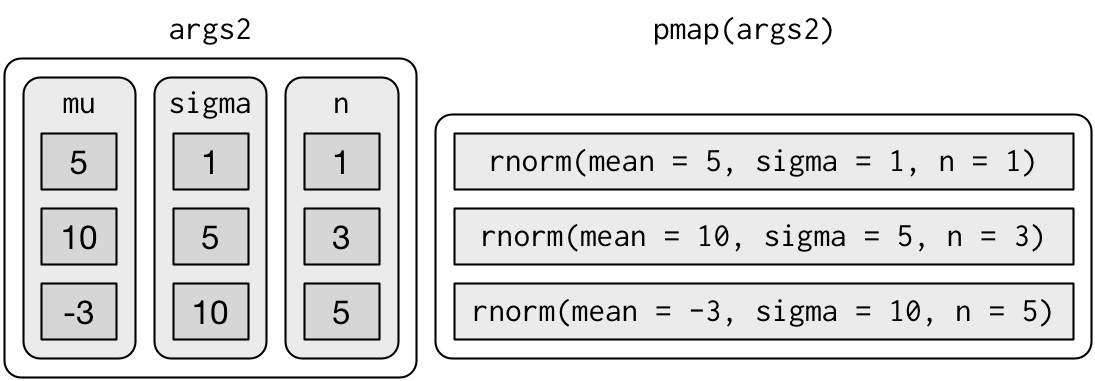
\includegraphics{../img/lists-pmap-named.png}
\caption{structure of pmap}
\end{figure}

\end{frame}

\begin{frame}[fragile]{これでもいいよ}

\begin{Shaded}
\begin{Highlighting}[]
\NormalTok{params <-}\StringTok{ }\KeywordTok{tribble}\NormalTok{(}
          \OperatorTok{~}\NormalTok{mean, }\OperatorTok{~}\NormalTok{sd, }\OperatorTok{~}\NormalTok{n,}
          \DecValTok{5}\NormalTok{,     }\DecValTok{1}\NormalTok{,   }\DecValTok{1}\NormalTok{,}
          \DecValTok{10}\NormalTok{,    }\DecValTok{5}\NormalTok{,   }\DecValTok{3}\NormalTok{,}
          \OperatorTok{-}\DecValTok{3}\NormalTok{,    }\DecValTok{10}\NormalTok{,  }\DecValTok{5}\NormalTok{)}
\NormalTok{params }\OperatorTok\StringTok{ }\KeywordTok{pmap}\NormalTok{(rnorm)}
\end{Highlighting}
\end{Shaded}

\begin{verbatim}
## [[1]]
## [1] 4.882609
## 
## [[2]]
## [1] 10.2085411 -0.3950189  4.3204454
## 
## [[3]]
## [1] -16.573692  15.466755   1.642132  -1.366528  -2.030175
\end{verbatim}

\end{frame}

\begin{frame}[fragile]{21.7.1 Involing different functions}

入力変数だけでなく処理する関数すら変えたい場合

\begin{block}{Notes!!}

現在\texttt{invoke\_map}は非推奨になっている。\texttt{exec}で代用するべしとある

\end{block}

\end{frame}

\begin{frame}[fragile]{\texttt{invoke\_map}}

関数名を文字列でわたす

\begin{Shaded}
\begin{Highlighting}[]
\NormalTok{f <-}\StringTok{ }\KeywordTok{c}\NormalTok{(}\StringTok{"runif"}\NormalTok{, }\StringTok{"rnorm"}\NormalTok{, }\StringTok{"rpois"}\NormalTok{)}
\NormalTok{param <-}\StringTok{ }\KeywordTok{list}\NormalTok{(}
          \KeywordTok{list}\NormalTok{(}\DataTypeTok{min =} \OperatorTok{-}\DecValTok{1}\NormalTok{, }\DataTypeTok{max =} \DecValTok{1}\NormalTok{), }
          \KeywordTok{list}\NormalTok{(}\DataTypeTok{sd =} \DecValTok{5}\NormalTok{), }
          \KeywordTok{list}\NormalTok{(}\DataTypeTok{lambda =} \DecValTok{10}\NormalTok{))}
\KeywordTok{invoke_map}\NormalTok{(f, param, }\DataTypeTok{n =} \DecValTok{5}\NormalTok{)}
\end{Highlighting}
\end{Shaded}

\begin{verbatim}
## [[1]]
## [1] -0.0002563163  0.0044804169  0.5215238971  0.6526673199 -0.2975950576
## 
## [[2]]
## [1] -8.0675832 -0.6323985  3.9644148  4.9581136  3.8533626
## 
## [[3]]
## [1] 11 11 11 12 14
\end{verbatim}

\end{frame}

\begin{frame}{Visualization of \texttt{invoke\_map}}

\begin{figure}
\centering
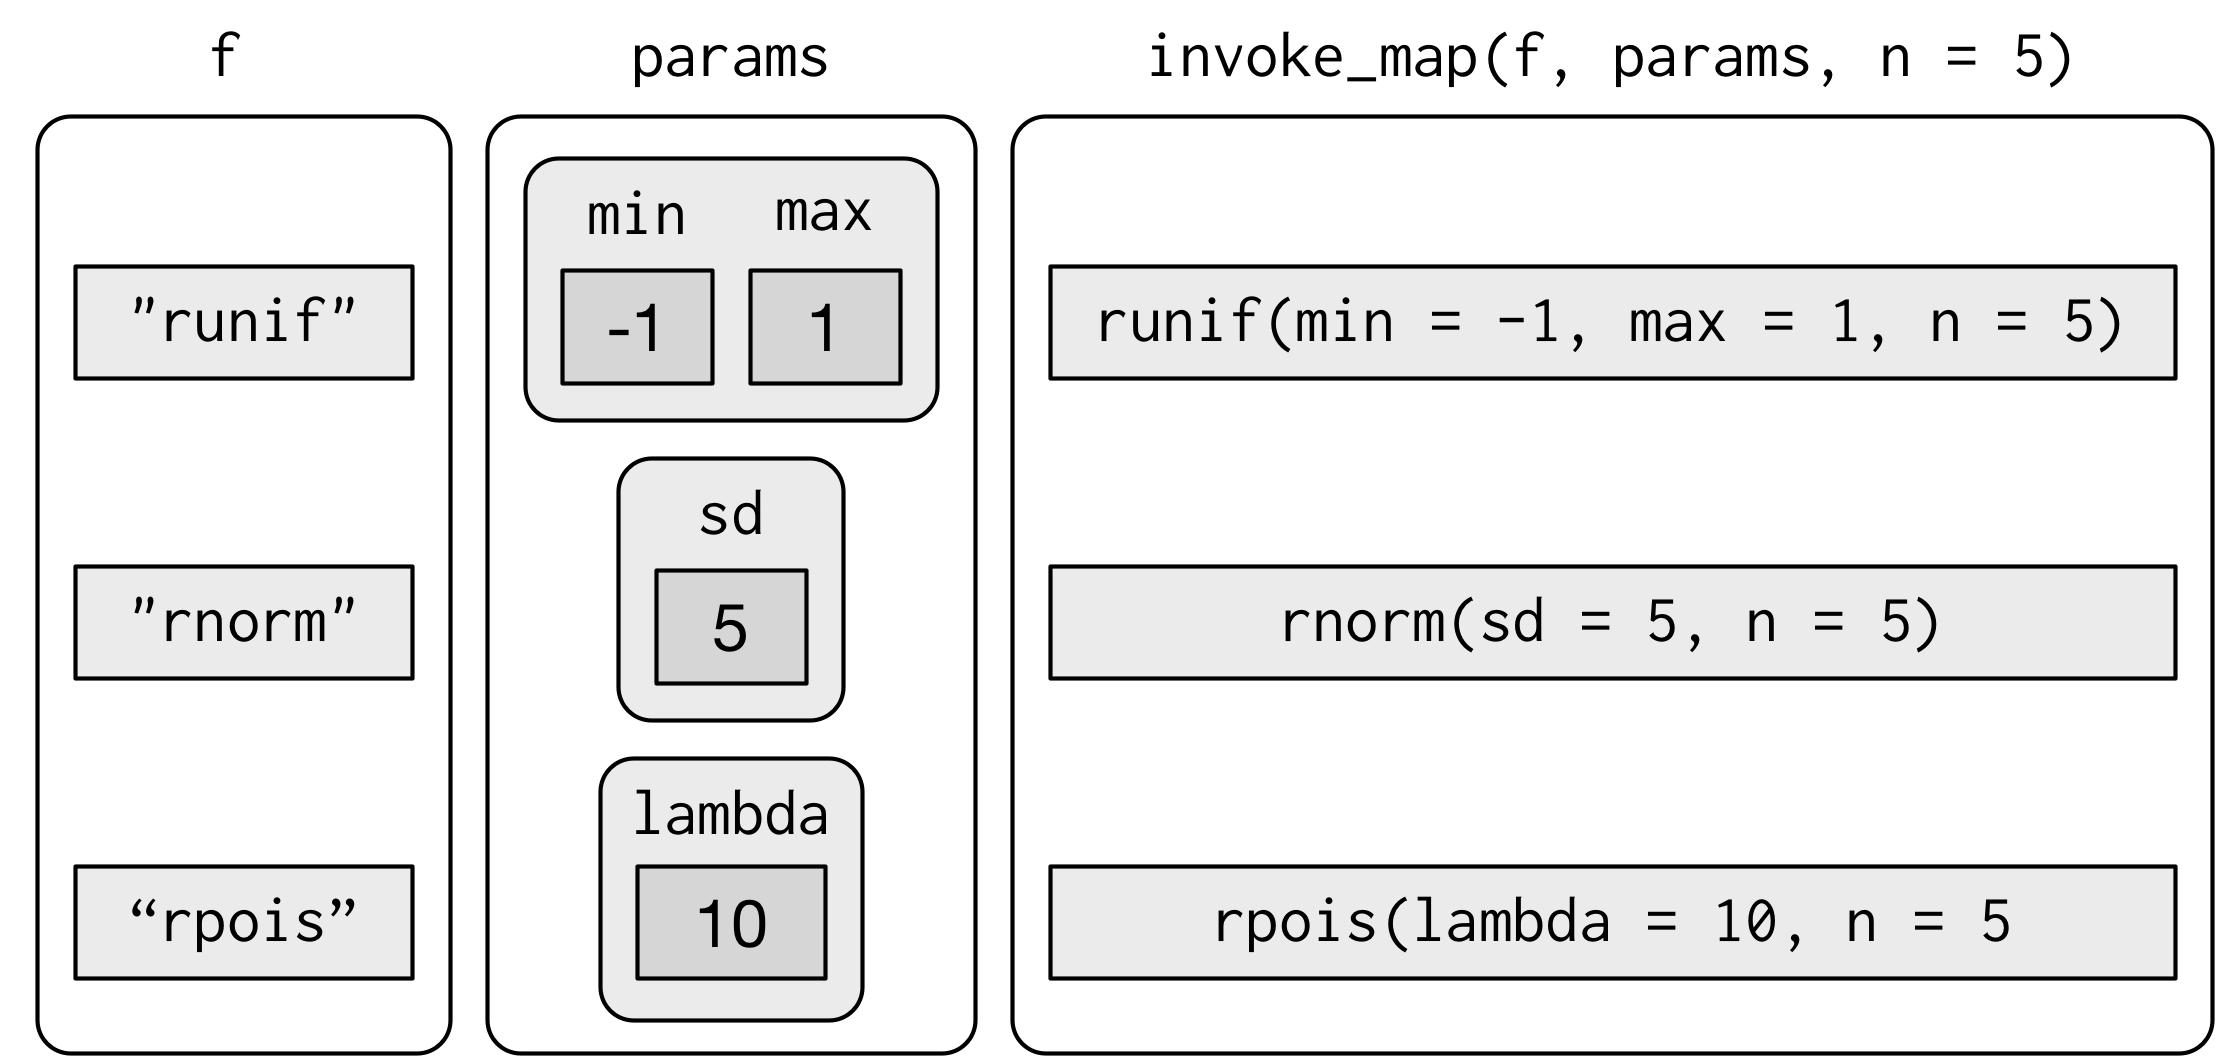
\includegraphics{../img/lists-invoke.png}
\caption{structure of invoke}
\end{figure}

\end{frame}

\begin{frame}[fragile]{\texttt{exec}で置き換え}

\begin{Shaded}
\begin{Highlighting}[]
\CommentTok{# Before:}
\KeywordTok{invoke_map}\NormalTok{(fns, }\KeywordTok{list}\NormalTok{(args))}
\KeywordTok{invoke_map}\NormalTok{(fns, }\KeywordTok{list}\NormalTok{(args1, args2))}

\CommentTok{# After:}
\KeywordTok{map}\NormalTok{(fns, exec, }\OperatorTok{!!!}\NormalTok{args)}
\KeywordTok{map2}\NormalTok{(fns, }\KeywordTok{list}\NormalTok{(args1, args2), }\ControlFlowTok{function}\NormalTok{(fn, args) }\KeywordTok{exec}\NormalTok{(fn, }\OperatorTok{!!!}\NormalTok{args))}
\end{Highlighting}
\end{Shaded}

\url{https://github.com/tidyverse/purrr/blob/master/NEWS.md\#retirement-of-invoke}

\end{frame}

\begin{frame}{21.8 Walk}

副作用を目的にFPを

\end{frame}

\begin{frame}[fragile]{\texttt{purrr::walk}}

\begin{Shaded}
\begin{Highlighting}[]
\NormalTok{x <-}\StringTok{ }\KeywordTok{list}\NormalTok{(}\DecValTok{1}\NormalTok{, }\StringTok{"a"}\NormalTok{, }\DecValTok{3}\NormalTok{) }

\NormalTok{x }\OperatorTok\StringTok{ }\KeywordTok{walk}\NormalTok{(print)}
\end{Highlighting}
\end{Shaded}

\begin{verbatim}
## [1] 1
## [1] "a"
## [1] 3
\end{verbatim}

\end{frame}

\begin{frame}[fragile]{\texttt{purrr::pwalk}}

\begin{Shaded}
\begin{Highlighting}[]
\NormalTok{plots <-}\StringTok{ }\NormalTok{mtcars }\OperatorTok\StringTok{ }
\StringTok{  }\KeywordTok{split}\NormalTok{(.}\OperatorTok{$}\NormalTok{cyl) }\OperatorTok\StringTok{ }
\StringTok{  }\KeywordTok{map}\NormalTok{(}\OperatorTok{~}\KeywordTok{ggplot}\NormalTok{(., }\KeywordTok{aes}\NormalTok{(mpg, wt)) }\OperatorTok{+}\StringTok{ }\KeywordTok{geom_point}\NormalTok{())}
\NormalTok{paths <-}\StringTok{ }\NormalTok{stringr}\OperatorTok{::}\KeywordTok{str_c}\NormalTok{(}\KeywordTok{names}\NormalTok{(plots), }\StringTok{".pdf"}\NormalTok{) }
\KeywordTok{pwalk}\NormalTok{(}\KeywordTok{list}\NormalTok{(paths, plots), ggsave, }\DataTypeTok{path =} \KeywordTok{tempdir}\NormalTok{())}
\end{Highlighting}
\end{Shaded}

\end{frame}

\begin{frame}[fragile]{21.9 Other patterns of for loops}

FPのバリエーション

\texttt{map}ほどは使わないが頭のどこかに置いておくといいことがあるかもしれない

\end{frame}

\begin{frame}{21.9.1 Predicate functions}

入力関数として出力が論理値の関数を受け付けて特殊な動作をする

\end{frame}

\begin{frame}[fragile]{\texttt{purrr::keep}と\texttt{purrr::discard}}

入力ベクトルの要素のうち、関数の判定が\texttt{TRUE}の要素のみを残す(捨てる)

入力がデータフレームなら\texttt{dplyr::select\_if}と同じ

\begin{Shaded}
\begin{Highlighting}[]
\NormalTok{iris }\OperatorTok\StringTok{ }\KeywordTok{keep}\NormalTok{(is.factor) }\OperatorTok\StringTok{ }\NormalTok{str}
\end{Highlighting}
\end{Shaded}

\begin{verbatim}
## 'data.frame':    150 obs. of  1 variable:
##  $ Species: Factor w/ 3 levels "setosa","versicolor",..: 1 1 1 1 1 1 1 1 1 1 ...
\end{verbatim}

\begin{Shaded}
\begin{Highlighting}[]
\NormalTok{iris }\OperatorTok\StringTok{ }\KeywordTok{discard}\NormalTok{(is.factor) }\OperatorTok\StringTok{ }\NormalTok{str}
\end{Highlighting}
\end{Shaded}

\begin{verbatim}
## 'data.frame':    150 obs. of  4 variables:
##  $ Sepal.Length: num  5.1 4.9 4.7 4.6 5 5.4 4.6 5 4.4 4.9 ...
##  $ Sepal.Width : num  3.5 3 3.2 3.1 3.6 3.9 3.4 3.4 2.9 3.1 ...
##  $ Petal.Length: num  1.4 1.4 1.3 1.5 1.4 1.7 1.4 1.5 1.4 1.5 ...
##  $ Petal.Width : num  0.2 0.2 0.2 0.2 0.2 0.4 0.3 0.2 0.2 0.1 ...
\end{verbatim}

\end{frame}

\begin{frame}[fragile]{\texttt{purrr::some}と\texttt{purrr::every}}

入力ベクトルの要素のうち、関数の判定がどれか(すべて)が\texttt{TRUE}なら\texttt{TRUE}

\begin{Shaded}
\begin{Highlighting}[]
\NormalTok{x <-}\StringTok{ }\KeywordTok{list}\NormalTok{(}\DecValTok{1}\OperatorTok{:}\DecValTok{5}\NormalTok{, letters, }\KeywordTok{list}\NormalTok{(}\DecValTok{10}\NormalTok{))}

\NormalTok{x }\OperatorTok\StringTok{ }\KeywordTok{some}\NormalTok{(is_character)}
\end{Highlighting}
\end{Shaded}

\begin{verbatim}
## [1] TRUE
\end{verbatim}

\begin{Shaded}
\begin{Highlighting}[]
\NormalTok{x }\OperatorTok\StringTok{ }\KeywordTok{every}\NormalTok{(is_vector)}
\end{Highlighting}
\end{Shaded}

\begin{verbatim}
## [1] TRUE
\end{verbatim}

\end{frame}

\begin{frame}[fragile]{\texttt{purrr::detect}}

条件が成立する最初の要素の値を返す。

\begin{Shaded}
\begin{Highlighting}[]
\NormalTok{x <-}\StringTok{ }\KeywordTok{sample}\NormalTok{(}\DecValTok{10}\NormalTok{)}
\NormalTok{x}
\end{Highlighting}
\end{Shaded}

\begin{verbatim}
##  [1] 10  9  5  3  1  8  7  6  4  2
\end{verbatim}

\begin{Shaded}
\begin{Highlighting}[]
\NormalTok{x }\OperatorTok\StringTok{ }\KeywordTok{detect}\NormalTok{(}\OperatorTok{~}\StringTok{ }\NormalTok{. }\OperatorTok{>}\StringTok{ }\DecValTok{5}\NormalTok{)}
\end{Highlighting}
\end{Shaded}

\begin{verbatim}
## [1] 10
\end{verbatim}

\begin{Shaded}
\begin{Highlighting}[]
\NormalTok{x }\OperatorTok\StringTok{ }\KeywordTok{detect_index}\NormalTok{(}\OperatorTok{~}\StringTok{ }\NormalTok{. }\OperatorTok{>}\StringTok{ }\DecValTok{5}\NormalTok{)}
\end{Highlighting}
\end{Shaded}

\begin{verbatim}
## [1] 1
\end{verbatim}

\end{frame}

\begin{frame}[fragile]{\texttt{purrr::head\_while}と\texttt{purrr::tail\_while}}

条件が成り立つまでの要素をすべて返す。

前から調べるか、後ろから調べるか

\begin{Shaded}
\begin{Highlighting}[]
\NormalTok{x }\OperatorTok\StringTok{ }\KeywordTok{head_while}\NormalTok{(}\OperatorTok{~}\StringTok{ }\NormalTok{. }\OperatorTok{>}\StringTok{ }\DecValTok{5}\NormalTok{)}
\end{Highlighting}
\end{Shaded}

\begin{verbatim}
## [1] 10  9
\end{verbatim}

\begin{Shaded}
\begin{Highlighting}[]
\NormalTok{x }\OperatorTok\StringTok{ }\KeywordTok{tail_while}\NormalTok{(}\OperatorTok{~}\StringTok{ }\NormalTok{. }\OperatorTok{>}\StringTok{ }\DecValTok{5}\NormalTok{)}
\end{Highlighting}
\end{Shaded}

\begin{verbatim}
## integer(0)
\end{verbatim}

\end{frame}

\begin{frame}{21.9.2 Reduce and accumulate}

2入力1出力関数のみを受け付ける特殊な関数

2つの入力の順序を入れ替えても出力の値が変わらない場合が望ましい

\end{frame}

\begin{frame}[fragile]{\texttt{purrr::reduce}}

\begin{Shaded}
\begin{Highlighting}[]
\NormalTok{dfs <-}\StringTok{ }\KeywordTok{list}\NormalTok{( }\DataTypeTok{age =} \KeywordTok{tibble}\NormalTok{(}\DataTypeTok{name =} \StringTok{"John"}\NormalTok{, }\DataTypeTok{age =} \DecValTok{30}\NormalTok{),}
        \DataTypeTok{sex =} \KeywordTok{tibble}\NormalTok{(}\DataTypeTok{name =} \KeywordTok{c}\NormalTok{(}\StringTok{"John"}\NormalTok{, }\StringTok{"Mary"}\NormalTok{), }\DataTypeTok{sex =} \KeywordTok{c}\NormalTok{(}\StringTok{"M"}\NormalTok{, }\StringTok{"F"}\NormalTok{)),}
        \DataTypeTok{trt =} \KeywordTok{tibble}\NormalTok{(}\DataTypeTok{name =} \StringTok{"Mary"}\NormalTok{, }\DataTypeTok{treatment =} \StringTok{"A"}\NormalTok{))}
\NormalTok{dfs }\OperatorTok\StringTok{ }\KeywordTok{reduce}\NormalTok{(full_join)}
\end{Highlighting}
\end{Shaded}

\begin{verbatim}
## Joining, by = "name"
## Joining, by = "name"
\end{verbatim}

\begin{verbatim}
## # A tibble: 2 x 4
##   name    age sex   treatment
##   <chr> <dbl> <chr> <chr>    
## 1 John     30 M     <NA>     
## 2 Mary     NA F     A
\end{verbatim}

\end{frame}

\begin{frame}[fragile]{\texttt{purrr::accumulate}}

\begin{Shaded}
\begin{Highlighting}[]
\NormalTok{x <-}\StringTok{ }\KeywordTok{sample}\NormalTok{(}\DecValTok{10}\NormalTok{)}
\NormalTok{x}
\end{Highlighting}
\end{Shaded}

\begin{verbatim}
##  [1]  6  4  5  3  1  2  8  7 10  9
\end{verbatim}

\begin{Shaded}
\begin{Highlighting}[]
\NormalTok{x }\OperatorTok\StringTok{ }\KeywordTok{accumulate}\NormalTok{(}\StringTok{`}\DataTypeTok{+}\StringTok{`}\NormalTok{)}
\end{Highlighting}
\end{Shaded}

\begin{verbatim}
##  [1]  6 10 15 18 19 21 29 36 46 55
\end{verbatim}

\end{frame}

\begin{frame}{21.9.3 Exercises}

頭の訓練に

\end{frame}

\end{document}
